\documentclass{foefyp}

\usepackage{lipsum}
\usepackage[utf8]{inputenc}
\usepackage[T1]{fontenc}
\usepackage{graphicx}
\usepackage{enumitem}
\usepackage{amsmath,amssymb,amsfonts}
\usepackage{multirow}% http://ctan.org/pkg/multirow
\usepackage{tabu}

% define Definition, Lemma, Theorem, Proof notation
\newtheorem{definition}{Definition}
\newtheorem{lemma}{Lemma}
\newtheorem{theorem}{Theorem}
\newtheorem{proof}{Proof}
% Macro list cuz im lazy to retype this
\newcommand\code[1]{$\texttt{#1}$}

\usepackage[backend=biber,style=ieee,sorting=none]{biblatex}
% TODO: edit to fit your own .bib file here
\addbibresource{cjason.bib}

% TODO: change to your own details
\author{Chia Jason}
\title{Design and Analysis for an Identity-Based Identification Scheme with Tight Security}
\submissionyear{2020}
\submissionmonth{January}
\faculty{Faculty of Engineering}
\degree{Bachelor of Engineering (Hons) Electronics majoring in Computer}
\studentID{1161300548}
\declareDate{Jan 01 2020} %Date to set at the declaration page

\begin{document}

\frontmatter
\makecoverandtitlepage
\copyrightpage
\declarationpage

\acknowledgements{Thanks to piky for this work.}

\abstractfromfile{abstract}

% TODO: fix your list of abbreviations
{\clearpage\SingleSpacing
\tableofcontents\clearpage
\listoftables\clearpage
\listoffigures\clearpage
\chapter{List of Abbreviations}
IBI\quad\quad Identity-Based Identification
\clearpage
}

\mainmatter

%!TEX ROOT = thesis.tex
\chapter{Introduction}

\section{Overview}
This section serves to guide readers into the project. It should generate interest and motivate readers to read further about the project. It should provide sufficient background for readers to understand the project’s problem statements. Usually, it is written by first describing the big picture of real life problems or scenarios and gradually narrows down to specific problems addressed by the project.

\section{Problem Statement}
This section serves to highlight the specific problems addressed by the project.

\section{Project Scope}
This section gives an overview of project activities, e.g. what are carried out, what are not and what the limitations are.

\section{Report Outline}
This section serves to inform readers about the organisation of the report, e.g. what are presented and where and how they are presented.

\subsection{Test SubSection}
Sample content in test subsection

\subsubsection{Test SubSubSection}
Sample content in test subsubsection \cite{tan11}


%!TEX ROOT = thesis.tex
\chapter{Literature Review}
This chapter demonstrates your ability to review, and to report on relevant literature and past work on your given topic. A well written literature review:

\begin{itemize}
	\item allows the reader to easily place the focus of your FYP project within the context of the wider academic community in your field;
	\item reports your critical review of the relevant literature; and
	\item identifies a gap within that literature that your research will attempt to address.
\end{itemize}

\section{Guides on Writing Literature Review}
What you need to do before writing your literature review:

\begin{enumerate}
	\item Find relevant literature on your FYP topic and follow streams of references
	\item Identify important themes/ideas/theories/approaches to the topic that have emerged during your research on your respective FYP topic
	\item Introduce ideas by themes/theory/approach/chronologically or any other appropriate structure but do not just list different authors’ viewpoints
	\item Introduce and explain each theme (or theory/approach), present evidence from readings (agreements/disagreements), critically commentate and relate to your own research
	\item Carefully note down each reference you intend to include in your literature review
\end{enumerate}

%!TEX ROOT = thesis.tex
\chapter{Details of the Design}
Sample figure and table here

\section{Figures and Tables}
\lipsum[1]

\begin{figure}[hbt!]\centering
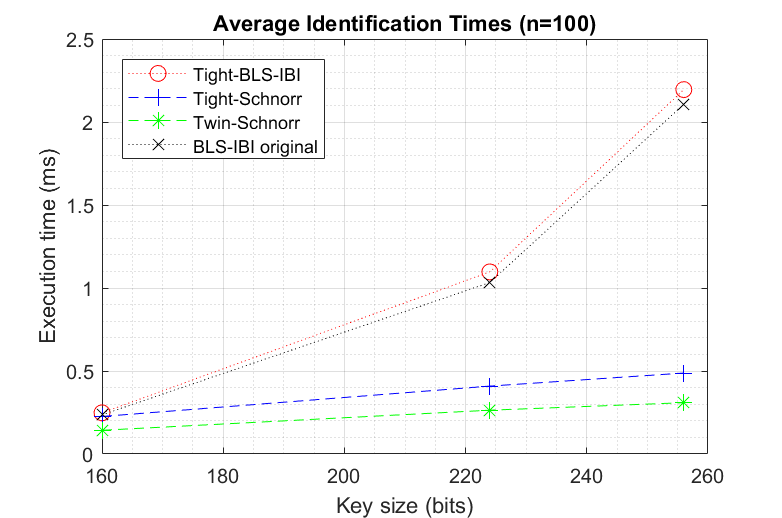
\includegraphics[width=\textwidth]{figures/nid2.png}
\caption{Some caption}
\end{figure}

\lipsum[5]

\begin{table}[hbt!]
\caption{This is a table}
\centering
\begin{tabular}{ l c r }
\hline
Hey & How's it & Going?\\ \hline
Fine! & Just great. & See ya!\\
Fine! & Just great. & See ya!\\
\hline
\end{tabular}
\end{table}



%!TEX ROOT = thesis.tex
\chapter{Data Presentation and Discussion of Findings}
The results/data presentation and discussion sections can be both the most interesting as well as the most challenging sections to write. You may choose to write these sections separately, or combine them into a single chapter, depending on your preferences.

\section{Data Presentation}
There are three main methods of presenting your data, be it the results of your experiments, information that you have collected and analysed, or statistics from secondary sources (such as books, journal articles or newspaper reports):

\begin{itemize}
    \item it can be incorporated into the main body of text;
    \item it can be presented separately as a table; or
    \item it can be used to construct a graph or chart.
\end{itemize}

\section{Sample algorithm}
\lipsum[2]
\begin{algorithm}
\caption{Euclid's algorithm}\label{euclid}
\begin{algorithmic}[1]
\Procedure{Euclid}{$a,b$}\Comment{The g.c.d. of a and b}
   \State $r\gets a\bmod b$
   \While{$r\not=0$}\Comment{We have the answer if r is 0}
      \State $a\gets b$
      \State $b\gets r$
      \State $r\gets a\bmod b$
   \EndWhile\label{euclidendwhile}
   \State \textbf{return} $b$\Comment{The gcd is b}
\EndProcedure
\end{algorithmic}
\end{algorithm}

\section{Sample Equation}

\lipsum[3]

\begin{align}
\label{eqn:soundness}
\begin{split}
	\frac{R_{SP_1}}{R_{SP_2}}^{\frac{1}{(C_{HA_1} - C_{HA_2})}} = \, & (\frac{ \delta^{ t+c_1 } }{ \delta^{ t+c_2 }})^{\frac{1}{(c_1 - c_2)}}  \\
	= \, &  (\delta^{c_1 - c_2})^{\frac{1}{c_1 - c_2}}  \\
	= \, &  \delta
\end{split}
\end{align}

%!TEX ROOT = thesis.tex
\chapter{Introduction}

\section{Overview}
This section serves to guide readers into the project. It should generate interest and motivate readers to read further about the project. It should provide sufficient background for readers to understand the project’s problem statements. Usually, it is written by first describing the big picture of real life problems or scenarios and gradually narrows down to specific problems addressed by the project.

\section{Problem Statement}
This section serves to highlight the specific problems addressed by the project.

\section{Project Scope}
This section gives an overview of project activities, e.g. what are carried out, what are not and what the limitations are.

\section{Report Outline}
This section serves to inform readers about the organisation of the report, e.g. what are presented and where and how they are presented.

\subsection{Test SubSection}
Sample content in test subsection

\subsubsection{Test SubSubSection}
Sample content in test subsubsection



\printbibliography[title=REFERENCES,heading=bibintoc]
\backmatter

\chapter{Appendix A}
Sample appendix


\end{document}
